\section{Introdução}

Este trabalho implementa um protocolo de comunicação customizado que não faz uso do protocolo TCP/IP.
As comunicações se dão via \textit{raw sockets} na camada 2 do modelo OSI \cite{osi_model}.
Nesse caso, utilizamos frames Ethernet II \cite{EthernetII}.
Os \textit{headers} (cabeçalhos) Ethernet são populados manualmente pelo sistema no seguinte formato:

\begin{figure}[H]
    \centering
    \begin{bytefield}[bitwidth=2.5em,boxformatting={\centering}]{14}
        \bitheader{0-13}\\
        \bitbox{6}{Destination MAC Address} &
        \bitbox{6}{Source MAC Address} &
        \bitbox{2}{Protocol}
    \end{bytefield}
    \caption{Header Ethernet II}
    \label{fig:eth2_header}
\end{figure}

\section{Definição do Protocolo}

O protocolo customizado, chamado de \lstinline{T1Protocol}, se baseia em: um tipo de mensagem, um campo de endereço, e um campo de dados.
O tipo de mensagem pode ser:

\begin{description}
    \hypertarget{proto_start}{}
    \item[START <NAME>] Mensagem enviada para o endereço de Broadcast, indicando que um novo nodo entrou na rede.
    O ``nome'' (\textit{name}) do nodo é seu endereço MAC.
    \hypertarget{proto_heartbeat}{}
    \item[HEARTBEAT <NAME>] Mensagem de \textit{alive} enviada via Broadcast para todos os nodos a cada 5 segundos, indicando que
    aquele dispositivo ainda está ativo na rede. O campo \textit{NAME} indica o endereço MAC do nodo que está enviando a mensagem.
    Essa mensagem também é utilizada ao receber uma mensagem do tipo \textit{START}. Nesse caso, é enviado um \textit{HEARTBEAT}
    diretamente ao nodo que enviou a mensagem de \textit{START}, e não ao endereço de Broadcast.
    \hypertarget{proto_talk}{}
    \item[TALK <NAME> <DATA>] Mensagem enviada quando um dispositivo deseja se comunicar com outros dispositivos via Broadcast.
    O campo \textit{NAME} contém o nome do dispositivo que está enviando a mensagem. O campo \textit{DATA} contém dados quaisquer.
\end{description}

O protocolo foi descrito na linguagem Protobuf 3 \cite{protobuf} para versioná-lo. Utilizamos o programa \textit{protoc} \cite{protoc} juntamente do programa \textit{betterproto} \cite{betterproto} para gerar as classes necessárias.

Todas as máquinas da rede possuem uma lista de roteamento (lista de máquinas conhecidas). Mensagens vindas de máquinas fora dessa
lista são ignoradas.
O sistema dispõe de uma maneira de remover máquinas automaticamente pelo tempo do último \textit{HEARTBEAT} de cada nodo.
Caso um nodo não envie um \textit{alive}/\textit{HEARTBEAT} por mais de 15 segundos, ele é removido da lista dessa máquina e dado como
offline. Para que ele seja adicionado novamente à lista do nodo atual, ele deve enviar uma mensagem de \textit{START}.

Sempre que uma máquina entra na rede e manda uma mensagem \textit{START}, os demais nodos adicionam essa nova máquina à suas listas de \textit{hosts} conhecidos/tabelas de roteamento e respondem-na diretamente com um \textit{HEARTBEAT}. A máquina que enviou o \textit{START} adiciona em sua lista de máquinas conhecidas todas as máquinas que responderam seu \textit{START} com um \textit{HEARTBEAT}.
A mensagem \textit{HEARTBEAT} enviada diretamente ao remetente que enviou o \textit{START} será chamada de \textit{ACK\_ALIVE} daqui em diante.

Não foi definido um limite máximo no tamanho dos dados na mensagem \textit{TALK}, então assumiu-se que os dados, juntamente dos headers e outras informações necessárias,
não ultrapassarão o tamanho máximo de um \textit{frame} Ethernet, \SI{1518}{\byte}.

As mensagens de \textit{HEARTBEAT} (para Broadcast) e \textit{START} não funcionariam corretamente sem o campo \textit{name}, que contém
o endereço MAC da máquina em si. Como a máquina de origem envia esses \textit{frames} para o endereço de Broadcast, os outros nodos
recebem o \textit{frame} como se estivesse sido enviada do endereço de Broadcast.
Acessando o campo \textit{name} podemos salvar o endereço MAC do nodo original e ignoramos o endereço de origem nesses casos

\section{Implementação Prática}

O trabalho foi escrito em Python 3.10 \cite{py310}, atual (\today) versão oficial da linguagem. 
Também utilizamos o sistema de descrição de protocolos Protobuf \cite{protobuf}/gRPC \cite{grpc}, da Google.

O relatório utiliza as palavras pacote, \textit{packet} e \textit{frame} para representar sempre um \textit{frame} Ethernet II.
Um ``pacote'' (\textit{packet}) só existe da camada 3 do modelo OSI \cite{osi_model} para cima.

\subsection{Protocolo}
\label{sec:protocolo}

Como mencionado acima, o protocolo foi definido na linguagem Protobuf 3 \cite{protobuf}.
O \textit{enum} \lstinline{MessageType} define o tipo de mensagem que será enviado, podendo ser um de:

\begin{itemize}
    \item \hyperlink{proto_start}{\lstinline{START}}
    \item \hyperlink{proto_heartbeat}{\lstinline{HEARTBEAT}}
    \item \hyperlink{proto_talk}{\lstinline{TALK}}
\end{itemize}

O campo \lstinline{type} do tipo \lstinline{MessageType} indica o tipo de mensagem daquele pacote.
O campo \lstinline{string name} contém o endereço MAC do remetente (a máquina que está enviando a mensagem).
O campo \lstinline{string data} contém os dados quaisquer que serão enviados na mensagem \hyperlink{proto_talk}{\textit{TALK}}.

\begin{figure}[H]
    \centering
\begin{minted}[xleftmargin=\parindent]{protobuf}
    syntax = "proto3";
    
    package t1_protocol;
    
    message T1Protocol {
        enum MessageType {
            START = 0;
            HEARTBEAT = 1;
            TALK = 2;
        }
        MessageType type = 1;
        string name = 2;
        string data = 3;
    }
\end{minted}
    \caption{Descrição do protocolo}
    \label{fig:protobuf_desc}
\end{figure}

Os frames enviados pelo sistema têm seu formato descrito pela \figurename{ \ref{fig:packet_format}}.

\definecolor{lightkhaki}{rgb}{0.94, 0.9, 0.55}

\begin{figure}[H]
    \centering
    \begin{bytefield}[bitwidth=3.5em,boxformatting={\centering}]{6}
        \bitheader{0-5}\\
        \begin{leftwordgroup}{Header}
        \bitbox{6}[bgcolor=lightkhaki]{Destination MAC Address} \\
        \bitbox{6}[bgcolor=lightkhaki]{Source MAC Address}\\
        \begin{rightwordgroup}{T1Protocol}
        \bitbox{2}[bgcolor=lightkhaki]{Protocol} & \bitbox{1}{Type} & \bitbox[lrt]{3}{}\end{leftwordgroup}\\
        \bitbox[lr]{6}{Name}\\
        \bitbox[lr]{6}{\tiny(\SI{17}{\byte})} \\
        \bitbox[lrb]{2}{} & \bitbox[rlt]{4}{}\\
        \bitbox[lr]{6}{Data \\ \tiny (dados de tamanho indeterminado)} \\
        \skippedwords \\
        \bitbox[lrb]{6}{}
        \end{rightwordgroup}
    \end{bytefield}
    \caption{Formato dos frames}
    \label{fig:packet_format}
\end{figure}

O tamanho máximo do campo \textit{Data} é de \SI{1486}{\byte}.

$$\SI{1518}{\byte}\text{ (max)} - \SI{14}{\byte}\text{ (header)} - \SI{1}{\byte}\text{ (type)} - \SI{17}{\byte}\text{ (name)} = \SI{1486}{\byte}$$

\subsection{Implementação}

O sistema consiste de uma interface simples via CLI e duas \textit{threads}, uma para recebimento de mensagens, e outra para envio de mensagens.
A thread de recebimento é uma instância da classe \lstinline{ReceiverDaemon}, que herda da classe \lstinline{RawSocketDaemon}.
A thread de envio é uma instância da classe \lstinline{SenderDaemon} que também herda de \lstinline{RawSocketDaemon}.

A classe \lstinline{RawSocketDaemon} define algumas propriedades comuns entre recebimento e envio como interface, endereço MAC e o objeto do socket em si.
A função \\\lstinline{create_and_bind_socket(iface: str)} cria e retorna o \textit{raw socket} com o protocolo \lstinline{ETH_P_ALL} (3) para
recebermos todos os pacotes da camada 2 e faz \textit{bind} à interface desejada.

\begin{figure}[H]
    \centering
\begin{minted}[xleftmargin=\parindent]{python}
    def create_and_bind_socket(iface: str) -> socket.SocketType:
        s = socket.socket(socket.AF_PACKET, socket.SOCK_RAW,
                          socket.htons(ETH_P_ALL))
        s.bind((iface, 0))
        return s
\end{minted}
    \caption{Criação do raw socket}
    \label{fig:create_and_bind_socket}
\end{figure}


Essa e outras funções de uso geral estão definidas no arquivo \path{src/socket_utils.py}, como
as funções de \lstinline{pack()} e \lstinline{unpack()} dos headers Ethernet.

\subsubsection{Os Daemons}

O \lstinline{ReceiverDaemon} é a classe que recebe dados do socket e que possui a tabela de roteamento
(\lstinline{self.known_hosts}) e cuida da lista de nodos ``vivos'' (\lstinline{self.alive_table}).
A thread possui um \textit{timer} que roda de 15 em 15 segundos que faz a verificação da lista de nodos ``vivos''.
Ao receber uma mensagem, a classe verifica se a mensagem é destinada ao seu MAC/Broadcast e, se sim, verifica se o remetente
está em sua lista de nodos conhecidos. Caso não esteja e a mensagem seja do tipo \textit{START} ou \textit{HEARTBEAT} com destino ao
seu MAC (e não ao Broadcast), a mensagem é processada (\figurename{ \ref{fig:match_data_type}}).

\begin{figure}[H]
    \centering
\begin{minted}[xleftmargin=\parindent]{python}
    match data.type:
        case T1ProtocolMessageType.START:
            # Salva nodo na lista de nodos conhecidos
            self.add_to_routing_table(data.name)
            # Responde com HEARTBEAT
            self.ack_alive(data.name)
        case T1ProtocolMessageType.HEARTBEAT:
            # Verifica se é uma resposta ao nosso START
            if src != sock_util.MAC_BROADCAST:
                self.add_to_routing_table(data.name)
            # Atualiza o tempo do último alive desse host
            self.update_alive_table(data.name)
        case T1ProtocolMessageType.TALK:
            # Imprime a mensagem recebida
            print(
                f'TALK[From {src} ({data.name}) to {dst}]: {data.data}')
            # Salva o último contato (para REDIAL)
            self.last_contact = data.name
        case _:
            print(f'Unknown type. Type: {packet_type}')
\end{minted}
    \caption{Processamento de mensagens}
    \label{fig:match_data_type}
\end{figure}

O \lstinline{SenderDaemon} é a classe que faz o envio de dados e é a responsável por enviar o um \textit{HEARTBEAT} e 5 em 5 segundos.
A classe possui uma fila do tipo \lstinline{Queue} para adição/remoção de comandos para que o sistema seja thread-safe.
O método \lstinline{SenderDaemon.put()} é quem faz a codificação dos dados da mensagem e adiciona na fila de processamento.
O \lstinline{put()} invoca o método \lstinline{encode_message()} para instanciar a classe \lstinline{T1Protocol} com os dados
da mensagem.

\begin{figure}[H]
    \centering
\begin{minted}[xleftmargin=\parindent]{python}
    def encode_message(self, type: T1ProtocolMessageType, data: str = '') -> T1Protocol:
        return T1Protocol(type=type, name=self.name, data=data)

    def put(self, type: T1ProtocolMessageType, dst: str, data: str = '') -> None:
        dest = [int(d, 16) for d in dst.split(':')]
        msg = self.encode_message(type, data)
        header = Header(pack_eth_header(self.mac_address, dest, ETH_CUSTOM_PROTOCOL))
        self.q.put((header, msg))
\end{minted}
    \caption{Inclusão na lista de mensagens}
    \label{fig:encode_put}
\end{figure}

No \textit{loop} dessa thread, ao receber uma mensagem, o header e mensagem são extraídos.
A mensagem é serializada para \textit{bytes} pelo método \lstinline{SerializeToString} do gRPC \cite{grpc}.
Então, é feito o envio do header somado com os dados serializados.

\begin{figure}[H]
    \centering
\begin{minted}[xleftmargin=\parindent]{python}
    def run(self) -> None:
        while True:
            message = self.q.get()
            header, proto_data = message
            proto_data = proto_data.SerializeToString()
            self.socket.send(header + proto_data)
\end{minted}
    \caption{Envio de mensagens}
    \label{fig:run_send}
\end{figure}

\section{Uso}

O programa possui um menu rudimentar que explica mais a fundo as opções, que são: 
\lstinline{MENU}, \lstinline{START}, \lstinline{HEARTBEAT}, \lstinline{TALK}, \lstinline{TALKTO}, \lstinline{REDIAL} e \lstinline{TABLE}.
As funções \lstinline{TALKTO} e \lstinline{REDIAL} são para aumentar a qualidade de vida do usuário, onde \lstinline{TALKTO} envia
para um ou mais destinos uma mensagem, e \lstinline{REDIAL} envia uma mensagem ao último nodo que nos enviou um \textit{TALK}.

Antes de rodar o programa é preciso instalar os pacotes necessários, de preferência em um ambiente virtual.

\begin{commandshell}
python3.10 -m venv venv && source venv/bin/activate
pip install -r requirements.txt
\end{commandshell}

Estando com o ambiente virtual habilitado, o programa pode ser invocado:

\begin{commandshell}
python main.py
\end{commandshell}

O programa também pode receber como argumento uma interface de rede para fazer o \textit{bind}:

\begin{commandshell}
python main.py $INTERFACE
\end{commandshell}

\section{Testes}

Utilizamos a arquitetura de rede demonstrada na \figurename{ \ref{fig:core_emu}} no CORE Emulator \cite{core_emu}.
Possuímos quatro nodos (\textit{n2}, \textit{n3}, \textit{n4} e \textit{n6}) conectados por uma switch.
Os endereços MAC dos nodos estão definidos na \tableautorefname{ \ref{tab:mac_addrs}}.

\begin{figure}[H]
    \centering
    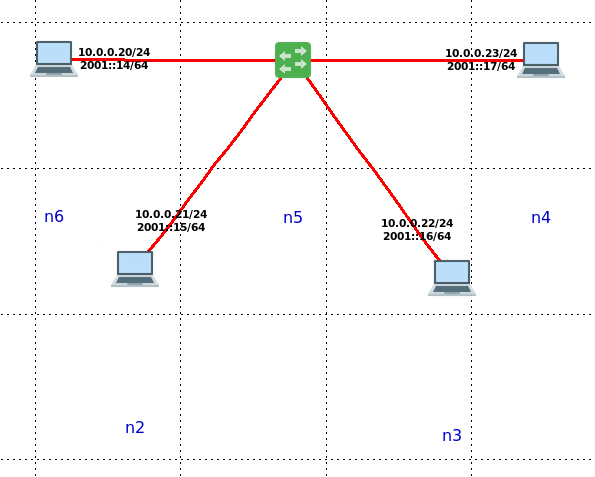
\includegraphics[width=30em]{CORE_EMU.png}
    \caption{Arquitetura da rede no CORE}
    \label{fig:core_emu}
\end{figure}

O nodo \textit{n5} é a switch de rede que faz a interconexão entre todos os nodos.

\begin{table}[H]
    \centering
    \begin{tabular}{cc}
        \textbf{Nodo} & \textbf{Mac} \\\hline
        n2 & 00:00:00:AA:00:01 \\
        n3 & 00:00:00:AA:00:02 \\
        n4 & 00:00:00:AA:00:03 \\
        n6 & 00:00:00:AA:00:00
    \end{tabular}
    \caption{Mapeamento de nodos para seus MACs}
    \label{tab:mac_addrs}
\end{table}

\begin{description}
    \item[START] Enviamos o \textit{START} apenas quando o usuário solicita. O \textit{START} é enviado usando a opção \textbf{1} ou \textbf{START} do menu. Demonstrado na \figurename{ \ref{fig:start_print}}.
    \begin{figure}[H]
        \centering
        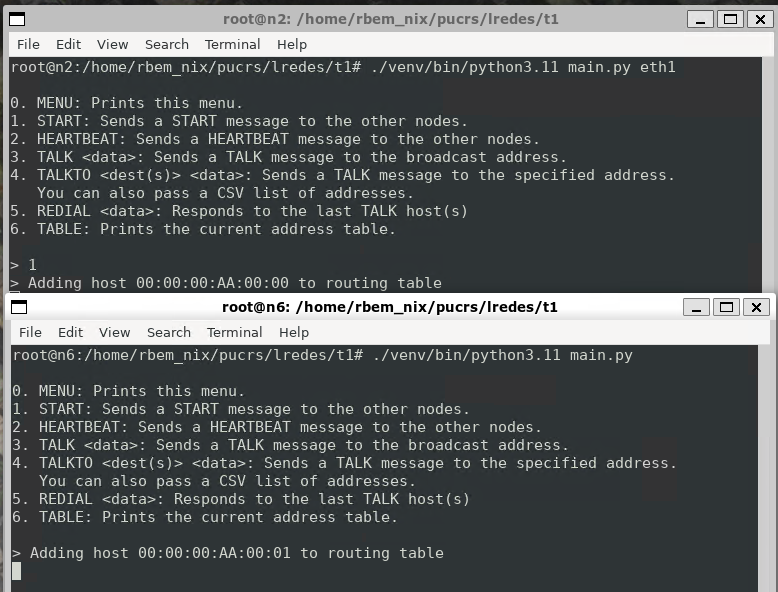
\includegraphics[width=30em]{START.png}
        \caption{START enviado por \textit{n2} e recebido por \textit{n6}}
        \label{fig:start_print}
    \end{figure}
    \item[HEARTBEAT de Resposta] Enviamos um \textit{HEARTBEAT} com destino ao nodo que nos enviou a mensagem de \textit{START}. Esse processo é feito de maneira autônoma e está demonstrado na \tableautorefname{ \ref{tab:heartbeat_start_print}}.
    \begin{table}[H]
        \centering
        \begin{tabular}{ccc}
            \textbf{Origem} & \textbf{Destino} & \textbf{Mensagem}\\\hline
            00:00:00:AA:00:02 & Broadcast & \textit{START}\\
            00:00:00:AA:00:00 & 00:00:00:AA:00:02 & \textit{HEARTBEAT}
        \end{tabular}
        \caption{\textit{START} enviado por \textit{n3}, recebido por \textit{n6} e respondido com \textit{HEARTBEAT}.\\
        Dados coletados com Wireshark \cite{wireshark}.}
        \label{tab:heartbeat_start_print}
    \end{table}
    \item[HEARTBEATS] Os nodos enviam um \textit{HEARTBEAT} para o endereço de Broadcast de 5 em 5 segundos.
    \item[Timeout] Passados 15 segundos sem receber um \textit{HEARTBEAT}, o nodo é removido da tabela de roteamento local.
    Essa funcionalidade está evidenciada na \figurename{ \ref{fig:heartbeat_timeout_print}}.
    \begin{figure}[H]
        \centering
        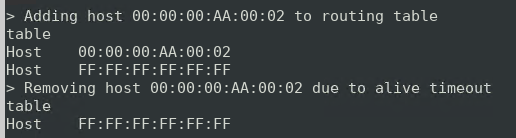
\includegraphics[width=30em]{TIMEOUT.png}
        \caption{Timeout de \textit{n3} em \textit{n6} por falta de \textit{HEARTBEAT}}
        \label{fig:heartbeat_timeout_print}
    \end{figure}
    \item[TALK] Mensagem enviada a todos os nodos via Broadcast com um payload de dados quaisquer.
    Demonstrado na \figurename{ \ref{fig:talk_print}}.
    \begin{figure}[H]
        \centering
        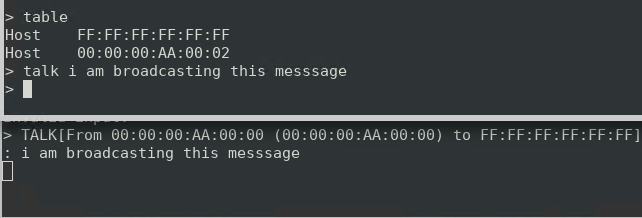
\includegraphics[width=30em]{TALK.png}
        \caption{\textit{TALK} de \textit{n6} para Broadcast, recebido por \textit{n3}}
        \label{fig:talk_print}
    \end{figure}
    \item[TALKTO] Envia um \textit{TALK} para um ou mais nodos diretamente, sem ser via Broadcast.
    A mensagem é definida por um ou mais endereços MAC separados por vírgula, seguidos de um espaço e os dados a serem enviados.
    \item[REDIAL] Envia um \textit{TALK} para o último nodo que nos contatou por último.
    Não faz nada quando não foi recebido um \textit{TALK} de outro nodo -- último contato está vazio.
\end{description}

\section{Conclusão}

Em suma, a utilização de raw sockets nos permite a utilização de protocolos diferentes, indo além dos clássicos TCP/IP e UDP.
Os \textit{frames} do protocolo \hyperref[sec:protocolo]{\lstinline{T1Protocol}} (definidos na \figurename{ \ref{fig:packet_format}}) são enviados diretamente pela segunda camada do modelo OSI \cite{osi_model}.
A ferramenta Wireshark \cite{wireshark} nos permitiu analisar os dados dos \textit{frames} enviados e recebidos e garantir que
o sistema funcione corretamente.
